\documentclass{eceasst}
% This is an empty ECEASST article that can be used as a template
% by authors.

% Required packages
% =================
% Your \usepackage commands go here.
\usepackage{graphicx}

\usepackage{listings}

\lstdefinestyle{myListingStyle} 
    {
        basicstyle = \small\ttfamily,
        breaklines = true,
    }

% Article frontmatter
% ===================
\title{FAIR4RS in Action: Lightweight Tooling for Computational Archaeology}

\author{
Florian Thiery\autref{1}\textsuperscript{,}\autref{*},
Lutz Schubert\autref{2},
Fiona Schenk\autref{3},
Peter Thiery\autref{4}}
\institute{
\autlabel{1} Research Squirrel Engineers Network \& Leibniz-Zentrum für Archäologie (LEIZA)\\
\autlabel{2} IT Center University of Cologne (ITCC)\\
\autlabel{3} Johannes Gutenberg-Universität Mainz\\
\autlabel{4} Research Squirrel Engineers Network, Limburgerhof\\
\autlabel{*} Correspondence: Florian Thiery, \email{florian.thiery@littleminions.link}\\}

\abstract{This paper presents a best-practice case study of FAIRification in Computational Archaeology through community-driven Research Software Engineering (RSE). Focusing on lightweight tools developed by the Research Squirrel Engineers Network, such as the SPARQLing Unicorn Toolkit and Jupyter Python Minions, we explore how FAIR4RS principles can be implemented in semantic workflows. Practical use cases from archaeology and geosciences – including Ogham stones and Campanian Ignimbrite sites – demonstrate how open, reusable code supports transparency, interoperability, and sustainability. The tools are critically discussed concerning the FAIR4RS and REAL (Reproducible, Executable, Attributable, Literal) frameworks, highlighting strengths and ongoing challenges. We argue that bottom-up RSE practices offer a viable path to sustainable, domain-specific FAIRification.}

\keywords{RSE, NFDI, Archaeology, FAIR, Open Science}

\newpage

\begin{document}
\maketitle

\section{Introduction}\label{sec:Introduction}

Archäoinformatik, internationally called Computational Archaeology, has become a crucial domain for demonstrating how Research Software Engineering (RSE)~\cite{homburg_recommendations_2021} contributes to developing sustainable, FAIR, and interoperable research workflows. The field combines archaeological theory with computational methods, working across geospatial modelling, semantic annotation, statistical analysis (e.g., using R and Python), and 3D data processing techniques such as photogrammetry and mesh reconstruction. Computational archaeology often requires scripting and automation, domain-specific semantic modelling, and the integration of heterogeneous data into semantically structured and machine-readable formats. In this context, research software is not merely an auxiliary layer  –  it is central to how archaeological knowledge is constructed, documented, and shared. Computational Archaeology is a prototypical use case for applying the FAIR principles to research software, known as FAIR4RS~\cite{barker_introducing_2022}, which aims to ensure that software is Findable, Accessible, Interoperable, and Reusable. Within the German National Research Data Infrastructure (NFDI), the role of RSEs is being formalised through initiatives such as the Working Group Research Software Engineering (INFRA-WG-RSE) of the Section Common Infrastructures~\cite{thiery_how_2025}. This group has developed a conceptual model describing three foundational pillars of RSE in digital infrastructures:

\begin{itemize}
    \item \textbf{Pillar I}: Research Software as Research Artefact: Software itself is treated as a scholarly output, requiring persistent identifiers, citation mechanisms, and long-term preservation strategies~\cite{katz_software_2016}
    \item \textbf{Pillar II}: Research Software as FAIRification Service: Software acts as an enabling layer in the semantic transformation and structuring of data according to FAIR principles, often incorporating linked data modelling and ontology alignment~\cite{schmidt_practices_2022,thiery_semi-automatic_2023}
    \item \textbf{Pillar III}: Research Software as Infrastructure Service: Mature tools become part of reusable infrastructure, so-called Basic services, offered by Base4NFDI, such as Jupyter4NFDI, or nfdi.software~\cite{bernard_base4nfdi_2023,team_base4nfdi_integration_2025}
\end{itemize}

These pillars (Figure~\ref{fig:001}) are accompanied by cross-cutting tasks: the creation of research software metadata, the implementation of quality criteria, contribution to long-term archiving and infrastructure provisioning, FAIR tool registration and discovery via nfdi.software, and the development of community guidelines and training programmes.

\begin{figure}[h!]
\centering
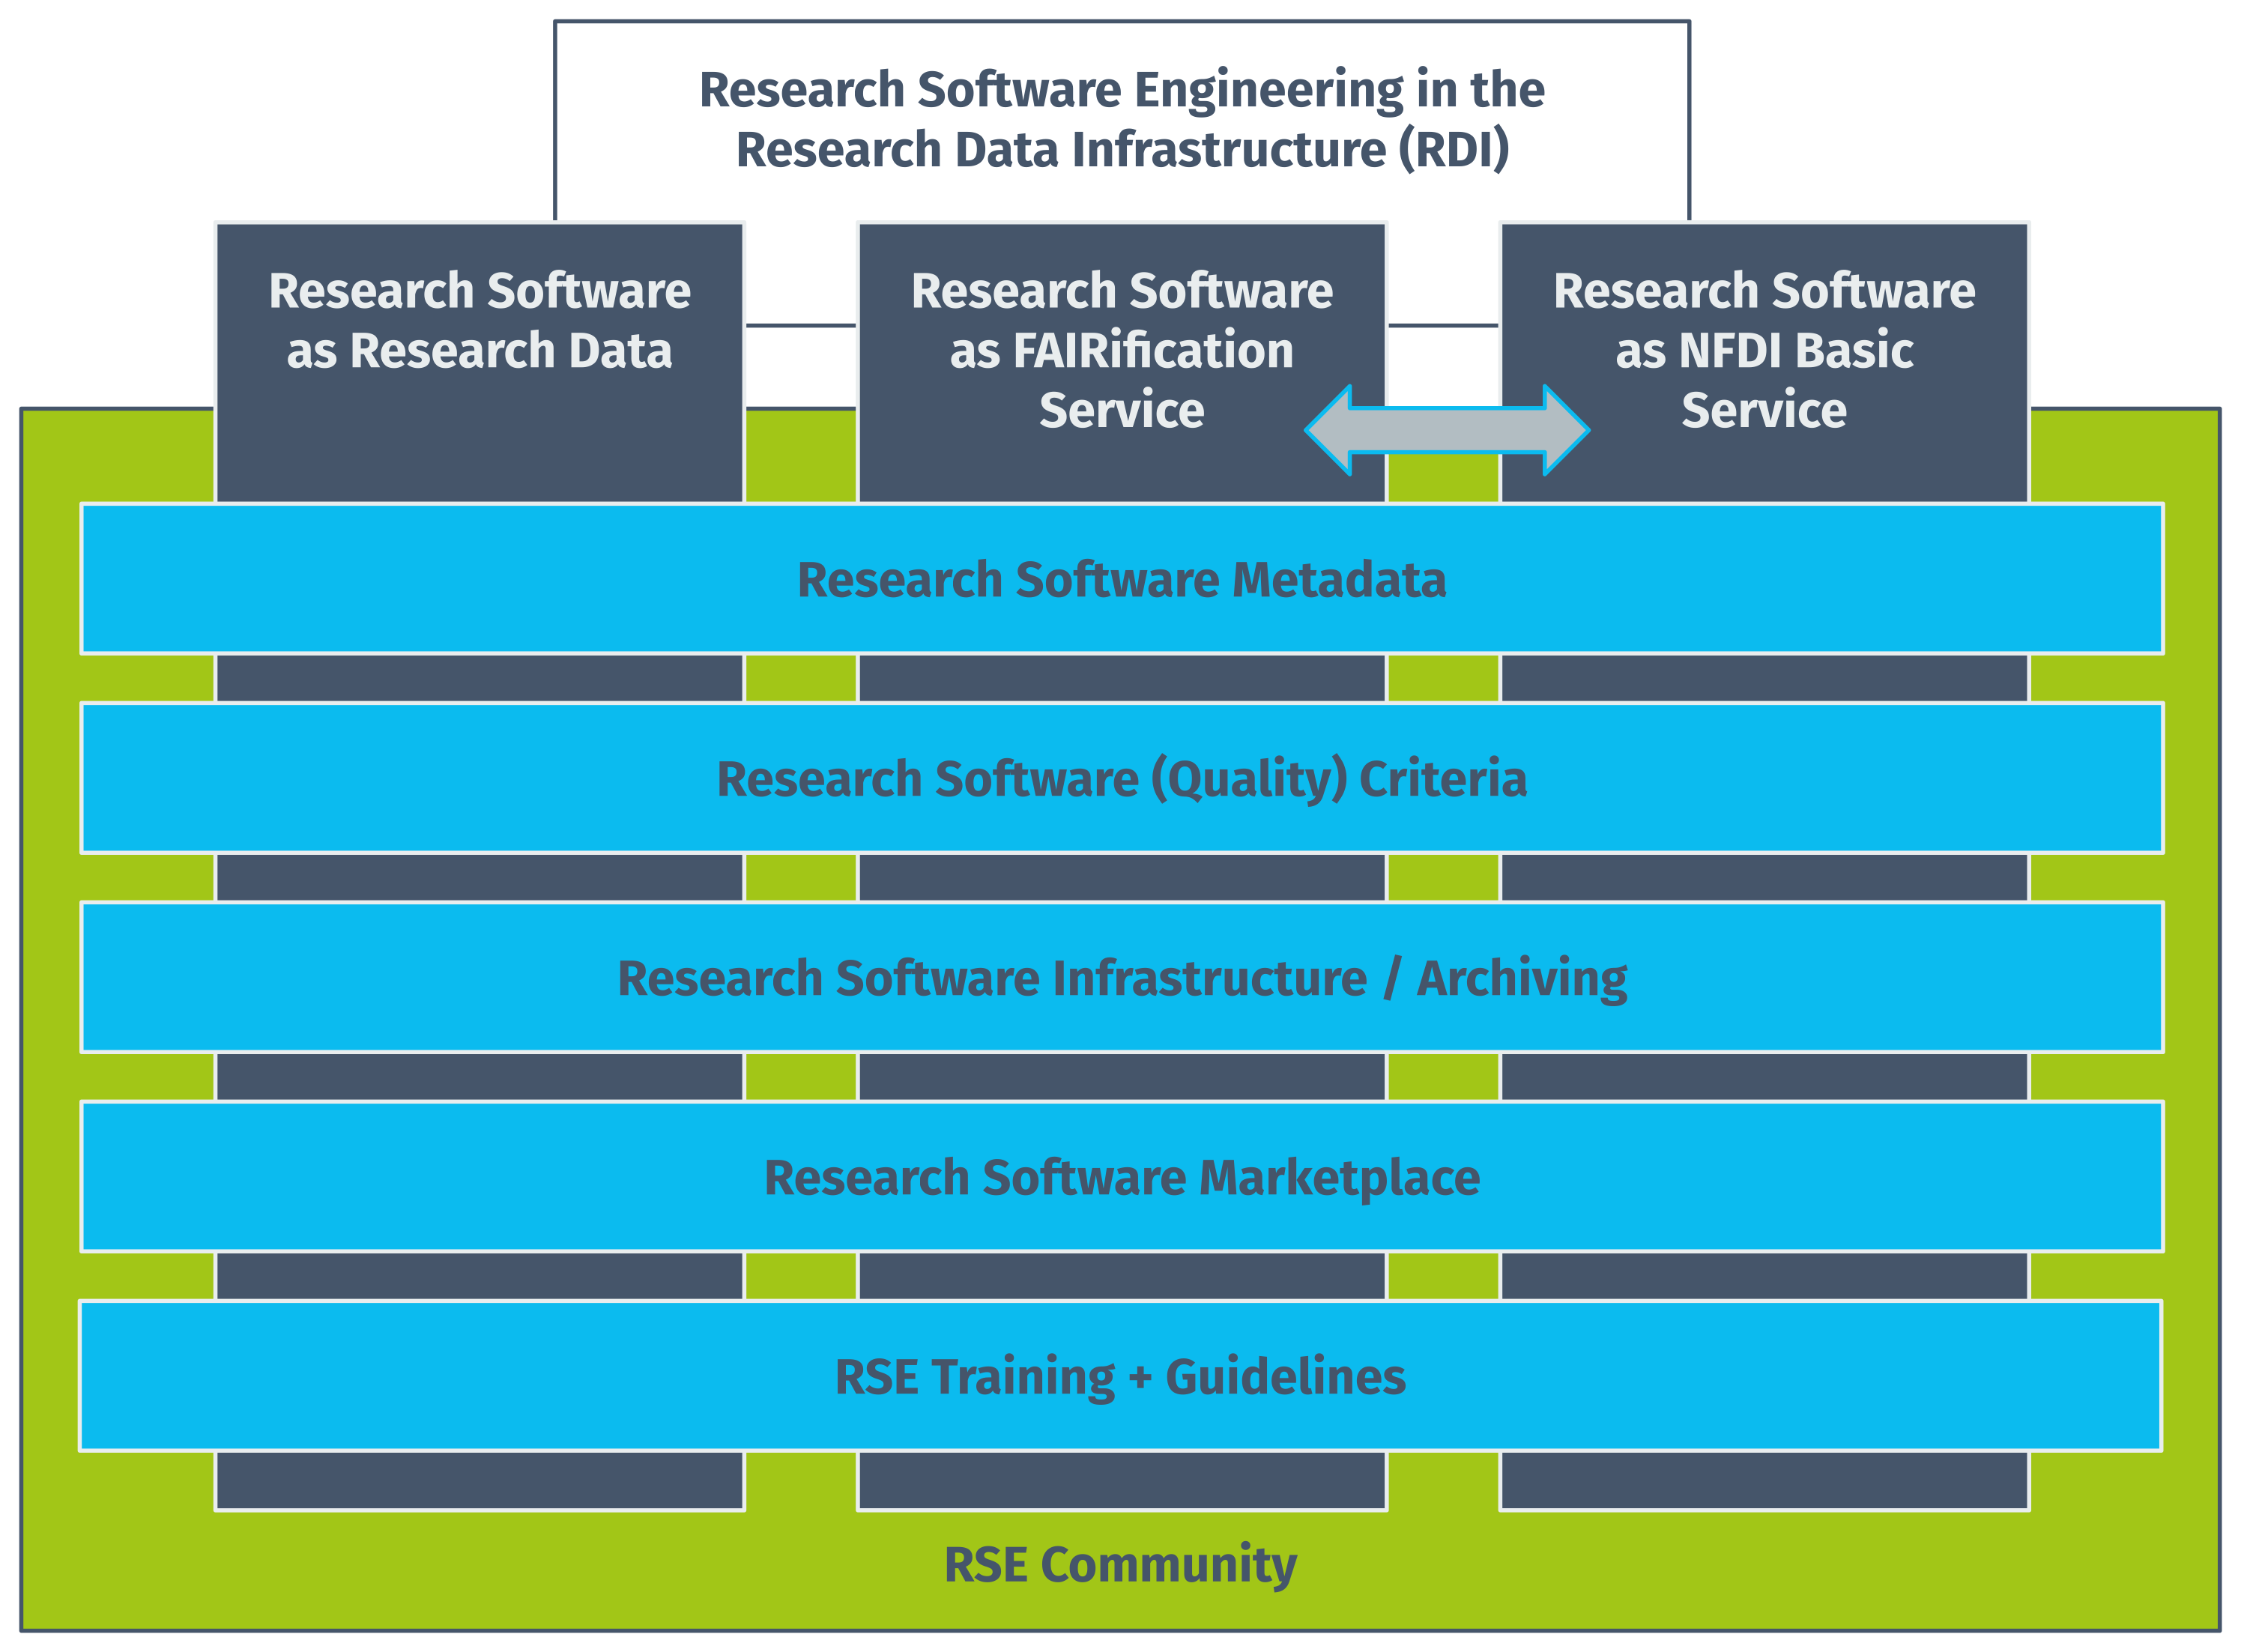
\includegraphics[width=0.95\linewidth]{ECEASST-LaTeX-Templates/img/Fig_03.png}
\caption{Schematic View on Research Software Engineering in the Research Data Infrastructure (RDI). Florian Thiery / INFRA-WG-RSE, CC BY 4.0.}\label{fig:001}
\end{figure}

A leading example of this approach in practice is the Research Squirrel Engineers Network, an informal community-of-practice founded in 2019. Its members are drawn from a variety of communities, including the German chapter of the Computer Applications and Quantitative Methods (CAA) community  –  CAA-DE  –  the CAA International SIG on Scientific Scripting Languages in Archaeology (SIG SSLA), and the Community Cluster Research Software Engineering of NFDI4Objects~\cite{thiery_digitale_2025,von_rummel_nfdi4objects_2025}. Together, they develop lightweight, modular Research FAIRification Tools (RFAIRTs), following the FAIR4RS principles and strongly emphasising interoperability, openness, and reusability.

These RFAIRT tools are – wihtin this paper – mostly embedded in the semantic web paradigm and rely on core technologies such as Linked Open Data (LOD), the Resource Description Framework (RDF), and (Geo)SPARQL. LOD refers to structured, interlinked data published in machine-actionable formats using RDF, enabling semantic interoperability across datasets~\cite{schmidt_practices_2022}. To query such data, so-called triplestores are used – specialised databases for storing RDF triples, accessed via the SPARQL query language. For geospatial contexts, GeoSPARQL extends SPARQL with spatial functions and geometry handling capabilities~\cite{car_geosparql_2022}.

While these technologies have been growing in digital humanities and computational archaeology, their application within Research Software Engineering (RSE) has remained limited, due to their steep learning curve and fragmented tooling. The SPARQLing Unicorn Research Toolkit addresses this gap by providing modular, accessible components that embed semantic data workflows into familiar research environments. In particular, tools like the Jupyter Python Minions, RDFier, and Academic Meta Tool (AMT) offer lightweight RSE-style entry points for creating, querying, and publishing LOD.

Exemplary RFAIRT tools are, e.g., the SPARQL Unicorn Research Toolkit~\cite{thiery_research_2025}, which include: (a) the SPARQLing Unicorn QGIS Plugin: a tool to send (Geo)SPARQL queries from QGIS to triple stores, transform QGIS vector layers into RDF, and document results as LOD-ready HTML, (b) the SPARQL Unicorn Ontology Documentation Tool enables GitHub-based workflows for automatic generation of ontology documentation as HTML files and (c) the Jupyter Python Minions: Reusable Python modules for querying semantic web sources from Jupyter Notebooks or scripts, and for visualising and analysing Linked Data. Additional FAIRification tools developed by the network include: (d) the RDFier: a CSV-to-RDF transformation engine for generating triplestore-ready data, (e) the Academic Meta Tool (AMT): a web-based utility for modelling vagueness and uncertainty in archaeological and geoscientific datasets, and (f) the Alligator: A chronologically aware classification tool, representing a use case of Pillar I: Research Software as Research Artefact.

These tools are documented and maintained openly, archived on platforms such as Zenodo, and integrated into central infrastructure services like: (i) Jupyter4NFDI, which supports the integration of Jupyter Notebooks as FAIR research objects, and (ii) nfdi.software, which acts as a software registry for discoverability, metadata, and reuse across consortia. The case of Computational Archaeology and the Research Squirrel Engineers exemplifies how domain-driven software development, grounded in open science and community collaboration, can deliver reusable infrastructure components. While the tools themselves are deeply rooted in the semantics and practices of archaeology and the geosciences, their design is intentionally generic enough to support transferability across domains, especially where Linked Open Data, uncertainty modelling, and geospatial integration are involved.

The presented software tools within this paper\footnote{This paper is based on the deRSE25 contributions IDs 9 (Research Squirrel Engineers: How an independent RSE-driven network may help the NFDI, \url{https://events.hifis.net/event/1741/contributions/13334/}), 137 (Keeping it REAL, \url{https://events.hifis.net/event/1741/contributions/13962/}), 8 (Squirrels und Unicorns - community-driven grassroots RSE-Lösungen zur FAIRification aus den Humanities \& Geosciences, \url{https://events.hifis.net/event/1741/contributions/14034/}), 108 (Jupyter Python Minion: Simplifying SPARQL Queries and Visualisations for Archaeological Data, \url{https://events.hifis.net/event/1741/contributions/13959/}), and 81 (Research Software Engineering in the NFDI), \url{https://events.hifis.net/event/1741/contributions/14053/})} have been developed and used within the activities of NFDI4Objects, CAA-DE, and the Special Interest Group on Scientific Scripting Languages in Archaeology (SIG SSLA\footnote{cf. \url{https://sslarch.github.io}}) presents the activities of the Research Squirrel Engineers as a best-practice model for implementing FAIR4RS in practice. The following chapters will examine the foundational motivation in sustainability challenges for Research Software in Computational Archaeology and the community-based development of RFAIRTs. The paper concludes with a broader discussion of how FAIR research software from Computational Archaeology can help shape sustainable and interoperable data infrastructures.

\section{Keeping it REAL - Sustainability Challenges for Research Software in Computational Archaeology}
\label{sec:REAL}

\paragraph{Is Reproducible Science REAL?} Open Science and Open Data are important elements for modern publications to make results FAIR and reproducible. This implies that any step involved in producing the data is equally made accessible - this includes any code used for analysis or data generation. Most authors will publish an algorithm or refer to a method rather than making the code available. Attempts to reproduce the results on this basis frequently lead to problems or deviations. For example when the method needs adaptation to the specific research question or the algorithm doesn't fit the data structure. To ensure verifiability of the paper, therefore, code must be treated in the same way as data, by making sure that all algorithmic processes published are

\begin{itemize}
    \item \textbf{Reproducible} in the sense that the results can be achieved again following all processes laid out in the paper without requiring additional steps that may be unclear or could lead to deviation
    \item \textbf{Executable} at any point in time - bearing compatibility problems in mind, this requires catering for the necessary containerization or virtualization
    \item \textbf{Attributable} to the data and author at the stage of publication, as well as any co-editor involved in creation of code, adaptation of data etc.
    \item \textbf{Literal} insofar as the algorithm is a sound and correct representation of the mathematical methods to be applied, and hence can lead to reproducable and generalisable results [the Turing way]
\end{itemize}

\begin{figure}[h!]
    \centering
    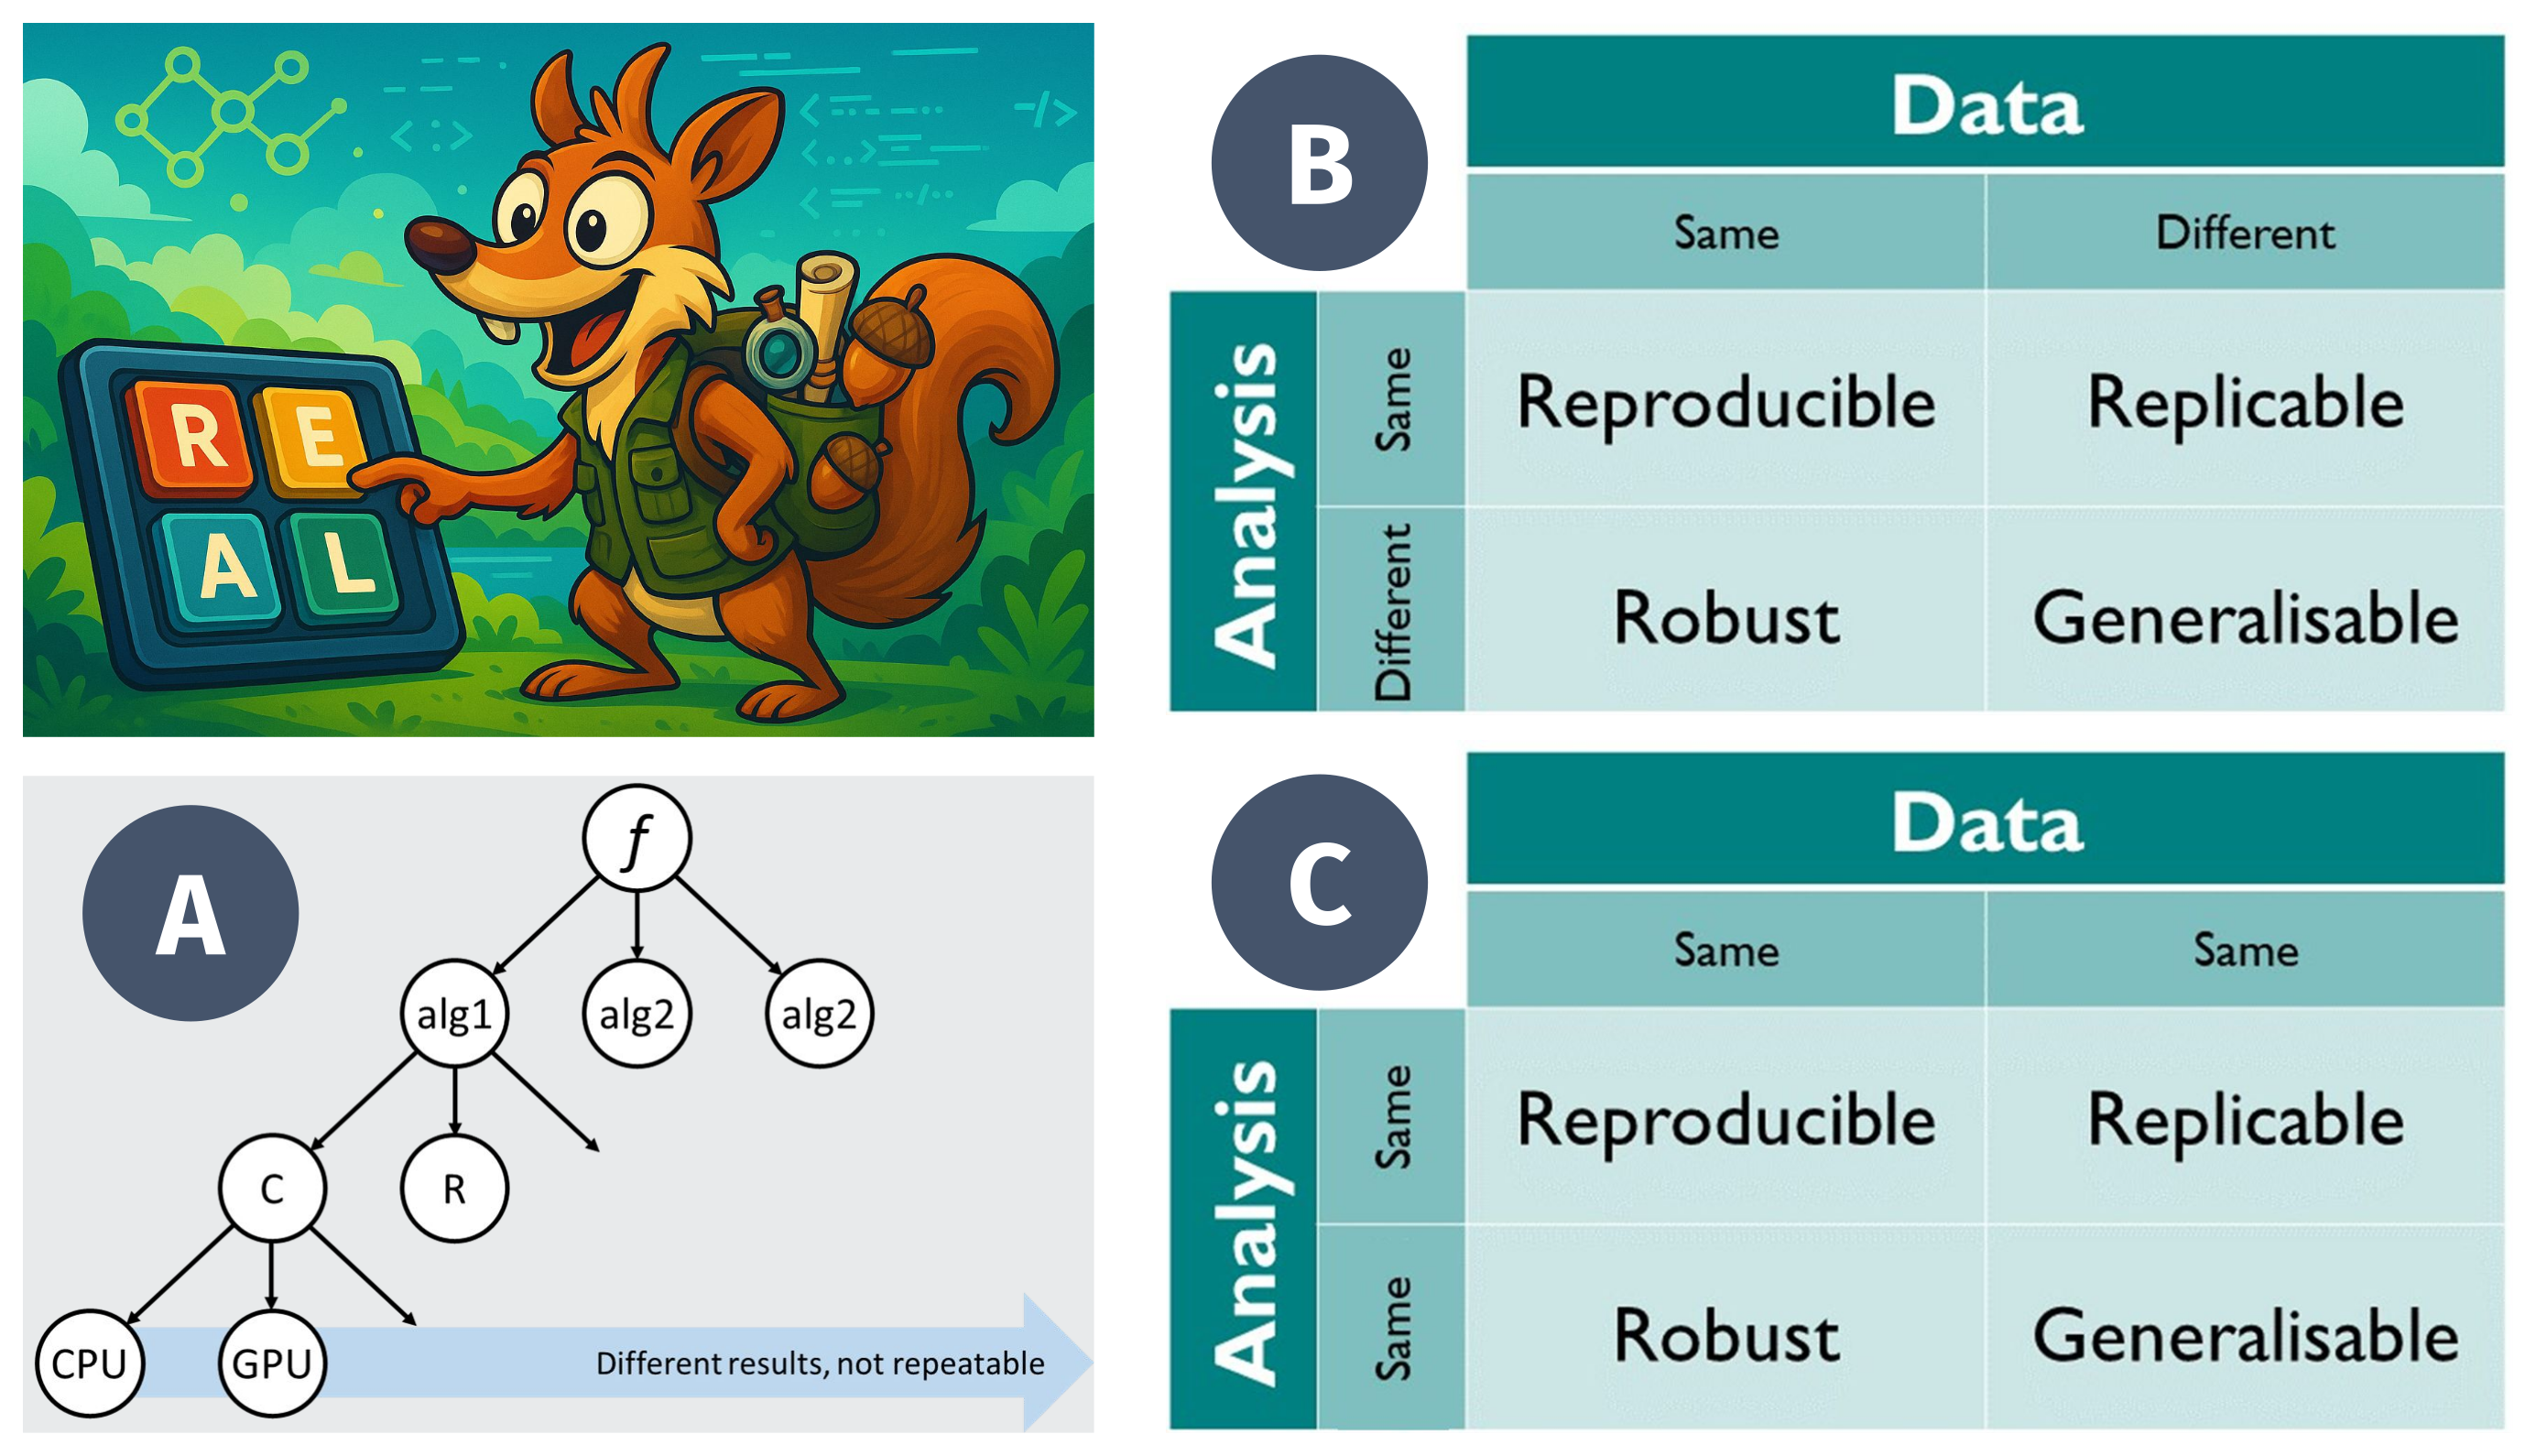
\includegraphics[width=0.95\linewidth]{ECEASST-LaTeX-Templates/img/REAL.png}
    \caption{Keeping it REAL. (A) Logical process from function to (running) code; (B) Reproducibility according to the Turing Way. Note how the conditions are extremely controlled; (C) Modified Turing Way. Note how the same conditions will lead to different interpretations of the results. top-left: Florian Thiery CC BY 4.0, created using OpenAI’s DALL·E; A-C: Lutz Krister Schubert, CC BY 4.0.}
    \label{fig:real}
\end{figure}

In general, scientists will generate their own code before reusing existing methods, primarily because of the complexity involved in (a) understanding existing code and (b) adapting it to the given needs. This means that code for the same functionality will be re-implemented repeatedly, making assessing its “Literal”ity difficult.  And even if two scientists have the same (mathematical) function in mind, they can choose different ways of realising and executing said function (Figure~\ref{fig:real}, A). A major problem consist in reproducibility over time. The same algorithm can lead to entirely different results depending on (1) choice of language, (2) data encoding, and (3) solver used (if needed)~\cite{hennessy_new_2019}. Similarly, and even worse, the same code can vary in results based on (1) the hardware it is executed on, (2) the compiler (settings) chosen, and (3) if solvers or AI are used, random coefficients. Because hardware, compilers and languages develop over time, the exact same code may not produce the same results anymore after 5 years.  Research Data Management, specifically archiving research software, typically supports long term reproducibility by virtualising the hardware and all components during code execution. This ensures that the same results can be reproduced, to a degree. In particular, where random parameters play a role in calculating the results, such as in Simulated Annealing, k-means or Monte Carlo methods, the same results can only be reproduced if the exact same random seeds are fed. In addition, effort, cost, and storage space are excruciating, limiting applicability seriously. Following the “Turing Way”, reproducibility is “\textit{when the same analysis steps performed on the same dataset consistently produces [sic!] the same answer}"~\cite{the_turing_way_community_turing_2025} strictly bound to the same data and the same type of analysis (aka code). As noted, though, very few algorithms, let alone codes, will create the exact same results unless under very controlled circumstances (Figure~\ref{fig:real}, B). What does that tell us, though? First of all, nothing else but that the code executes. After all: 

\begin{lstlisting}[
    style = myListingStyle,
    caption = {}
    ]
    void main(){return rnd();}
\end{lstlisting}

As we can see, the strict Turing Way definition - and therefore the generally acknowledged definition of FAIR and Open Science Code, namely to be fully reproducible - does not lead to actual insights into the code's correctness (i.e. “Literal”ity). We take it for granted by noting that code and data are accessible. However, we are really interested in a publication's scientific relevance and validity - in other words, whether the results apply to a broader range of conditions. Or, to put it in terms of the Turing Way, if they are generalisable. This is immediately obvious with methods such as Monte Carlo or k-means, which rely on stability over random parameters. The implicit statement of such an analysis differs from Reproducibility and is closer to Replicability and Robustness of the Turing Way. Yet, we need to bear in mind that data and analysis have not changed. Instead, as depicted in (Figure~\ref{fig:real}, C), they \textit{stay the same, yet lead to different results}. We therefore distinguish between different Interpretability of the results in terms of:

\begin{itemize}
    \item \textbf{Reproducible}: data, code and all environmental conditions are identical. Interpretation of the results is limited to the conditions applied
    \item \textbf{Replicable / Robust}: the results differ per execution, but stay within the expected tolerance. In other words, the interpretation of the results is unchanged. 
    \item \textbf{Generalisable}: even if all conditions are varied, the results stay within the expected boundaries. Accordingly, the interpretation can only be that the assumption is universally applicable. 
\end{itemize}

In the future we must clearly identify the degree of tolerance the interpretation of results allows. In other words, a good REAL publication provides not only all relevant data \textit{and} code, but also an assessment of the scope of validity of the results. In some cases this requires serious re-thinking of the interpretation.

\section{Community-driven grassroots Research FAIRification Tools (RFAIRT) coded from Humanities and Geosciences}\label{Sec31}

The development and maintenance of FAIR-compliant research software is increasingly shaped not only by institutional infrastructures but also by small, agile communities of practice (CoP). In computational archaeology, where research data are often diverse in format, analogue in origin, and rich in contextual uncertainty, domain-specific solutions are needed to support FAIRification in a practical and sustainable way. 

This section introduces such an approach through the concept of Research FAIRification Tools (RFAIRT)  –  lightweight, modular, community-driven software artefacts designed to implement the FAIR principles within archaeological and geoscientific workflows. The term RFAIRT refers to open, reproducible research tools that support the semantic transformation, querying, publication, and visualisation of data in accordance with FAIR and FAIR4RS principles. These tools are not generic infrastructure services, but demonstrators  –  proof-of-concept applications that enable and exemplify domain-embedded FAIRification. Their strength lies in their adaptability, low technical barriers, and ability to be embedded within existing workflows and widely adopted environments, such as QGIS and Jupyter Notebooks. 

At the centre of this ecosystem stands the Research Squirrel Engineers Network with the SPARQL Unicorn idea~\cite{thiery_sparql_2020}, a grassroots collective of Linked Open Data enthusiasts, research software engineers, archaeologists, geoscientists, and citizen scientists. Founded in 2019, the network grew out of the desire to connect heritage data with semantic web technologies in a transparent, collaborative, and sustainable manner. Since then, it has produced a growing portfolio of RFAIRTs, including the SPARQLing Unicorn Research Toolkit, the Jupyter Python Minions, and complementary tools such as RDFier and AMT (Academic Meta Tool)~\cite{unold_academic_2019}. 

The network is strongly connected to broader initiatives such as the CAA Germany, the Special Interest Group on Scientific Scripting Languages in Archaeology (SIG-SSLA) of CAA International, and the Community Cluster RSE within NFDI4Objects. Its development philosophy reflects a bottom-up, domain-sensitive logic: tools are created by those who need them. They are designed to work with the data and software environments already used in day-to-day research. The FAIRification processes are therefore grounded in practice, not abstraction. Crucially, these RFAIRTs do not only aim to make data FAIR, but also the code itself – according to the FAIR for Research Software (FAIR4RS) principles. This includes findability (persistent identifiers and registries like nfdi.software), accessibility (open licensing), interoperability (standardised formats, SPARQL, RDF), and reusability (clear documentation, modular structure). Furthermore, they respond to the challenges outlined in the REAL framework introduced in section 2: the tension between reproducibility and real-world conditions, the fragility of execution environments, the difficulty of attributing software contributions, and the complexity of preserving algorithmic clarity (Literalness) over time. Rather than aspiring to create universal solutions, the RFAIRTs produced by the Research Squirrel Engineers serve as working blueprints – reusable, adaptable, and open examples of how semantic FAIRification can be realised in Computational Archaeology. They focus on demonstrating pathways, fostering interoperability, and offering starting points for other researchers or communities wishing to align their tools and data with FAIR principles.

\subsection{Concept and Community – RFAIRT as FAIRification Demonstrators}\label{sec:31}

The comprehensible and collaborative collection and FAIRification of research data is becoming increasingly important within citizen science and digital heritage communities. Especially in domains like archaeology and the geosciences, semantic FAIRification of heterogeneous data is often driven by individuals and informal groups rather than large-scale infrastructures. These efforts are nonetheless crucial for integrating research data into broader federated ecosystems such as NFDI4Objects, Wikidata, OpenStreetMap, and the NFDI Knowledge Graph Infrastructure (KGI4NFDI). Within this context, the Research Squirrel Engineers Network is a community-of-practice focused on developing and applying FAIRification demonstrators – modular, open-source tools that implement LOD principles using accessible software stacks and everyday research practices. The network grew from efforts to prototype the SPARQLing Unicorn Research Toolkit, and has since evolved into a collective that connects grassroots semantic web development with national research infrastructure agendas. The tools developed by Squirrels  –  particularly the SPARQLing Unicorn QGIS Plugin and the Jupyter Python Minions – address the need for lightweight, reusable semantic integration workflows. These tools lower the barrier for researchers to: (a) access and query semantic data from triplestores, Wikibases, and Solid Pods, (b) transform archaeological or geoscientific data into RDF using established ontologies, (c) document and visualise these data in human- and machine-readable formats; and (d) embed FAIRification directly into common digital workflows (GIS, Python, Jupyter). By operating at the intersection of software, data, and community, these tools exemplify the principles of FAIR4RS while remaining rooted in real-world research needs. They are not intended to be universal platforms, but pragmatic demonstrators – tools that work, evolve through use, and serve as entry points for others. In the following subchapters, two of these demonstrators will be presented in detail. Section 3.2 introduces the SPARQLing Unicorn Research Toolkit, a set of QGIS- and GitHub-based tools for semantic integration and publication of archaeological and geoscientific Linked Data. Section 3.3 presents the Jupyter Python Minions, a set of lightweight scripts to support Linked Data querying and visualisation in Jupyter Notebooks. Together, they illustrate how FAIRification can be enacted from the bottom up – and how Research Software Engineering, when practised collaboratively, becomes a driver for sustainable Open Science.

The development of the described tools within this paper follows open, community-driven practices. Code repositories are publicly available on GitHub, typically under the respective accounts of the Research Squirrel Engineers Network members. In these projects, decisions about new features, pull request merging, and bug fixing are made collaboratively by the core developers and active contributors. For example, the SPARQLing Unicorn QGIS Plugin is maintained through its public issue tracker GitHub Issues\footnote{example SPARQLing Unicorn QGIS Plugin: \url{https://github.com/sparqlunicorn/sparqlunicornGoesGIS/issues}}, which documents user feedback, feature requests, and development milestones. New releases are regularly published and assigned persistent identifiers (DOIs) via Zenodo. Metadata, contributor roles, and citation information are described using the Citation File Format (CFF). While there is no formalised governance board, project leadership and maintainership emerge organically from sustained contributions within the network.

\subsection{The SPARQLing Unicorn Research Toolkit}\label{sec:32}

The SPARQLing Unicorn Research Toolkit emerged in 2019 from a simple but pressing challenge: how can researchers in Computational Archaeology and related disciplines meaningfully interact with LOD sources in their existing digital workflows, especially within the geospatial context of QGIS? Over time, this challenge gave rise to a modular and open set of FAIRification demonstrators, designed to bridge the semantic web and GIS environments and make linking and reusing research data transparent and repeatable. The toolkit's core is the SPARQLing Unicorn QGIS Plugin, developed within the Research Squirrel Engineers Network. This tool enables users to perform three main functions within a familiar GIS interface:

\begin{itemize}
    \item (A) Query external LOD sources using (Geo)SPARQL directly from within QGIS, for example, from Wikidata, the NFDI4Objects Knowledge Graph, or a Solid Pod
    \item (B) Transform local QGIS vector data into RDF, using ontologies such as GeoSPARQL or CIDOC CRM-aligned vocabularies
    \item (C) Export and document results as Linked Data HTML pages, using automated GitHub Actions workflows based on RDF files
\end{itemize}

These functionalities allow archaeologists, geoscientists, and digital humanists to visualise, transform, and publish semantically enriched data with minimal overhead, while adhering to the FAIR4RS principles. The toolkit is open source, versioned, archived, and actively maintained by a volunteer community. While this ensures accessibility and reusability, long-term sustainability depends on continued community engagement – a reality that ties directly into the REAL principles discussed in section 2.

\paragraph{Use Case 1 – Ogham Stones.} The SPARQLing Unicorn Research Toolkit has been successfully applied to the Linked Open Ogham project, which aims to make early medieval Ogham inscriptions FAIR and semantically interlinked. Ogham, an Early Medieval alphabet used between the 4th and 7th centuries AD, provides key insights into early Irish society's genealogical, linguistic, and territorial dimensions. The toolkit enables the querying, transformation, and publication of epigraphic metadata derived from digitised sources such as the Corpus Inscriptionum Insularum Celticarum (CIIC), historical Ordnance Survey maps, excavation reports, and museum documentation. These heterogeneous data sources are transformed into RDF, stored in triplestores, e.g. NFDI4Objects, Wikidata, fuzzy-sl Wikibase~\cite{thiery_linked_2023}, and accessed directly in QGIS through SPARQL queries executed via the plugin (Figure~\ref{fig:unicorn_ogham}). The plugin supports transforming vector data (e.g. findspot points, excavation layers) into RDF, preserving both geospatial and semantic attributes. In parallel, the HTML documentation generator – using GitHub Actions – creates human- and machine-readable metadata pages for each object. One examples is CIIC 178 (Coumeenole North / Dunmore Head): This stone, inscribed with ERC MAQI MAQI-ERCIAS-MU DOVINIA, is located near a promontory fort and associated with layered historical features, including a reported engraved cross. The site is documented as RDF and visualised in QGIS, allowing researchers to explore its strategic spatial context concerning other ritual and territorial markers. The HTML output links to secondary literature and includes properties such as fsl:certaintyLevel and fsl:hasReference for interpretive transparency.

\begin{figure}[h!]
    \centering
    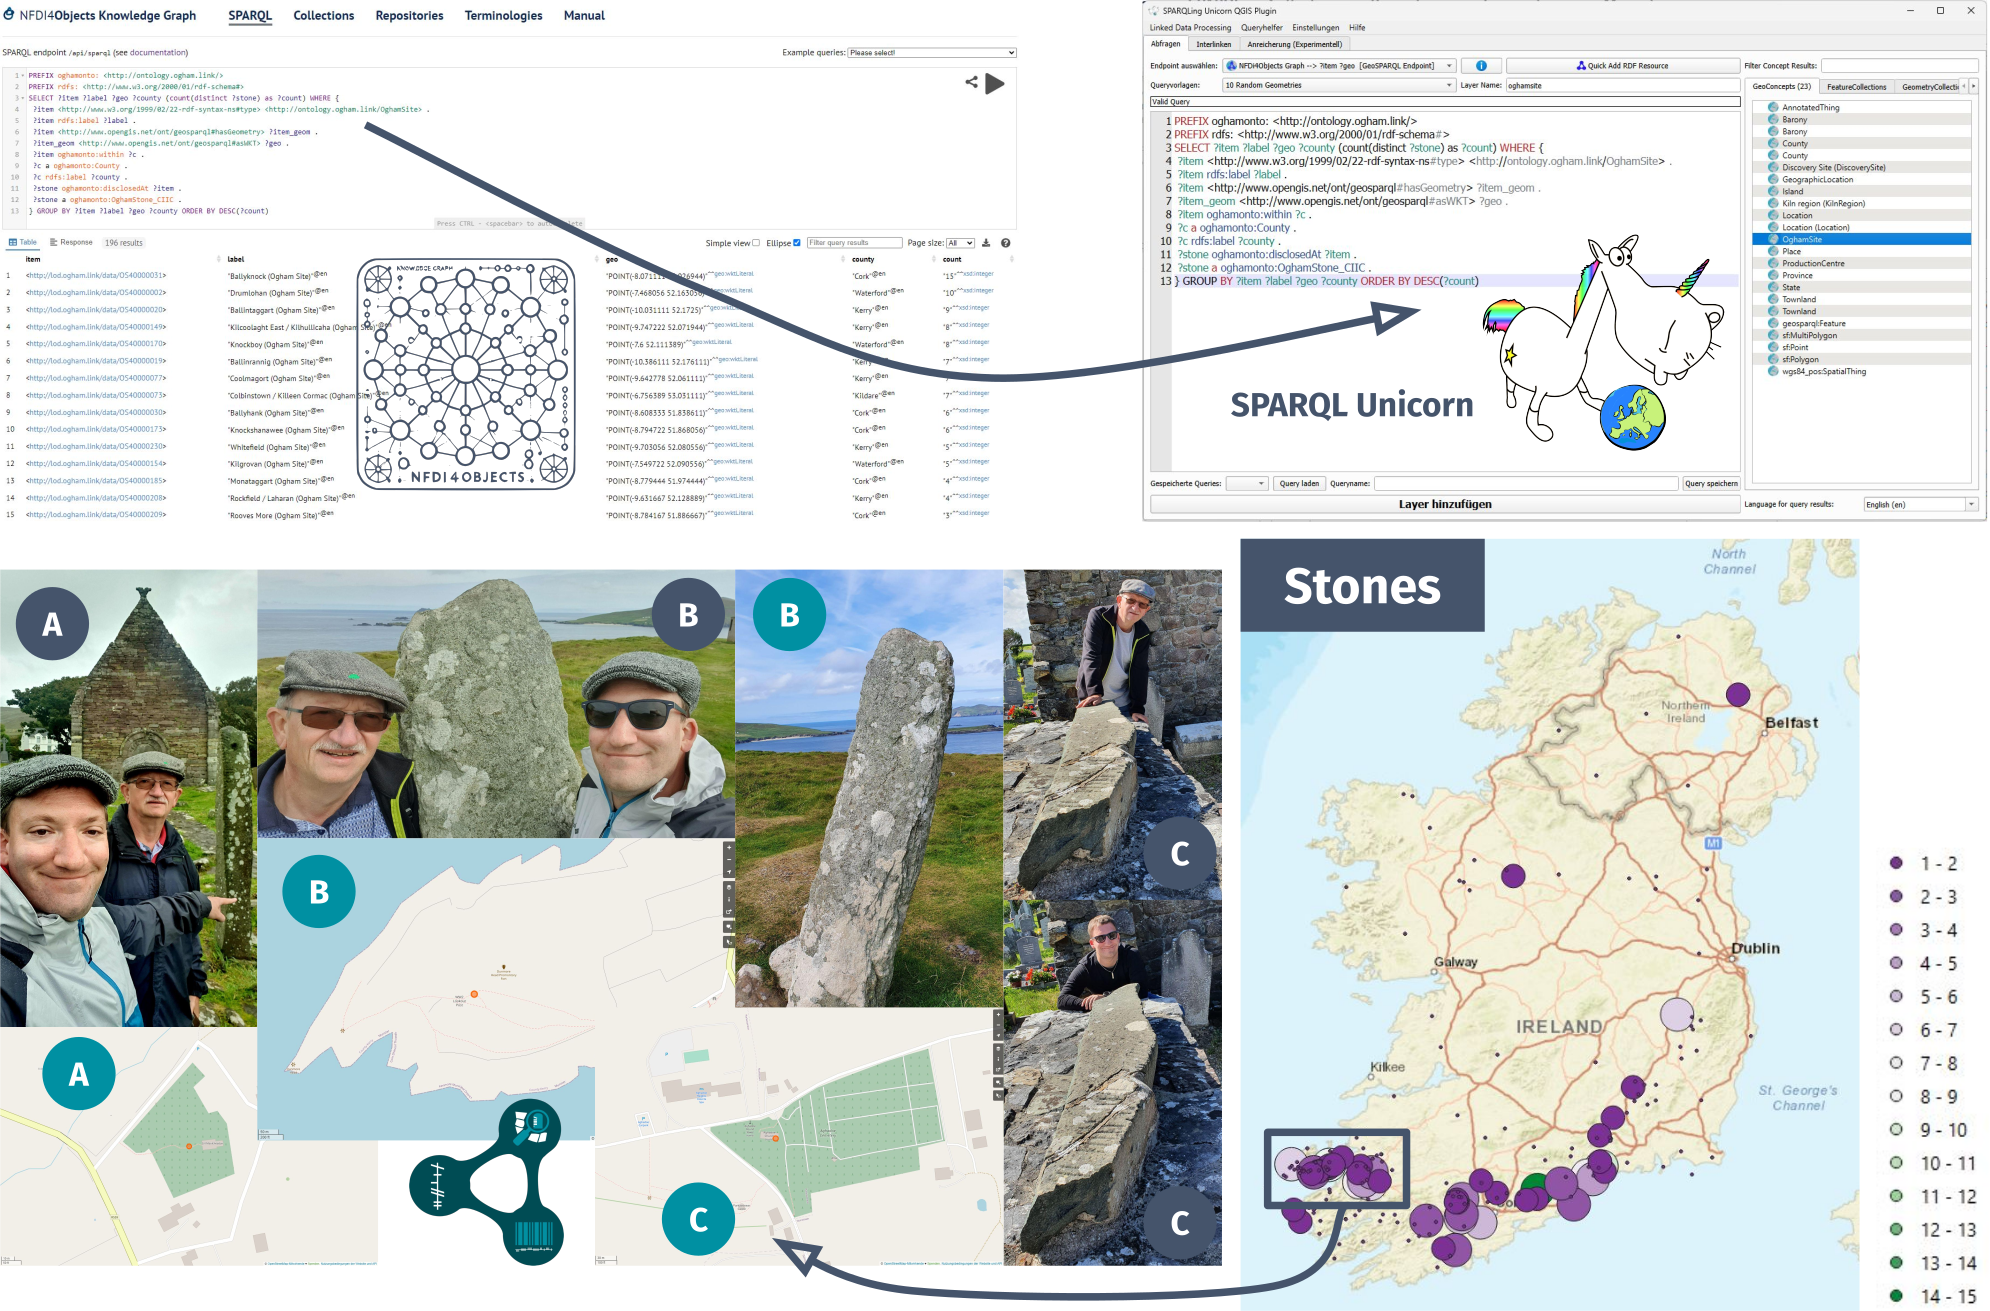
\includegraphics[width=0.95\linewidth]{ECEASST-LaTeX-Templates/img/Ogham KG Unicorn.png}
    \caption{Schema for visualising a query of the NFDI4Objects Knowledge Graph for Irish Ogham stones, their county and quantity, via \href{https://t1p.de/v0lg7}{https://t1p.de/v0lg7}, using the SPARQLing Unicorn QGIS Plugin and Ogham Stones on the Dingle Peninsula. Unicorn figures: Florian Thiery, CC BY 4.0; images: Florian \&Peter Thiery, CC BY 4.0; maps: (c) OpenStreetMap contributors.}
    \label{fig:unicorn_ogham}
\end{figure}

\paragraph{Use Case 2 – Campanian Ignimbrite.} The second demonstrator highlights the interdisciplinary applicability of the toolkit. It focuses on geoscientific and archaeological sites associated with the Campanian Ignimbrite (CI) eruption – Europe’s most powerful volcanic event of the Late Pleistocene, ca. 39,940 yr b2k ± 150 years~\cite{schenk_cryptotephra_2024}. While of interest to archaeological chronologies, these sites are also essential for tephrochronology, palaeoclimatology, and geochemistry. A key dataset includes stratified core samples from Auel Maar (AU3/4) and Dehner Maar (DE3) in the Eifel region of Germany. Schenk et al. (2024) documented that cryptotephra layers identified in the Auel Maar sediments were geochemically matched with CI/Y-5 tephra deposits found as far southeast as Urluia, Romania. This supports the hypothesis of a far-reaching fallout plume and provides evidence for CI-derived volcanic glass distribution across central Europe. In this interdisciplinary use case, the SPARQLing Unicorn Toolkit was used to: transform core metadata, especially geolocation, into RDF, query and visualise these data layers in QGIS, using Solid Pod storage and SPARQL endpoints as data sources, and document the information in semantically structured HTML pages (Figure~\ref{fig:unicorn_ci}), each with stable and resolvable URIs: Auel Maar AU3 (fsl:cisite\_201), Auel Maar AU4 (fsl:cisite\_202) and Dehner Maar DE3 (fsl:cisite\_203); these sites are also semantically linked to Wikidata items: Auel Maar (Q134466471) and Dehner Maar (Q134466523). The dataset includes archaeologically significant cave sites, such as Franchthi Cave (fsl:cisite\_45) and Toplitsa Cave (fsl:cisite\_44). In both cases, cryptotephra from the CI eruption has been detected within archaeological stratigraphy. These examples clearly show how geoscientific findspots often coincide with archaeological sites, reinforcing the importance of interdisciplinary collaboration and semantic alignment in data modelling. The toolkit fosters a cross-domain research infrastructure by enabling spatial visualisation, semantic linkage, and Linked Data publication of these sites. RDF-based representation ensures interoperability, while HTML documentation and GitHub workflows support transparency and versioning.

\begin{figure}[h!]
    \centering
    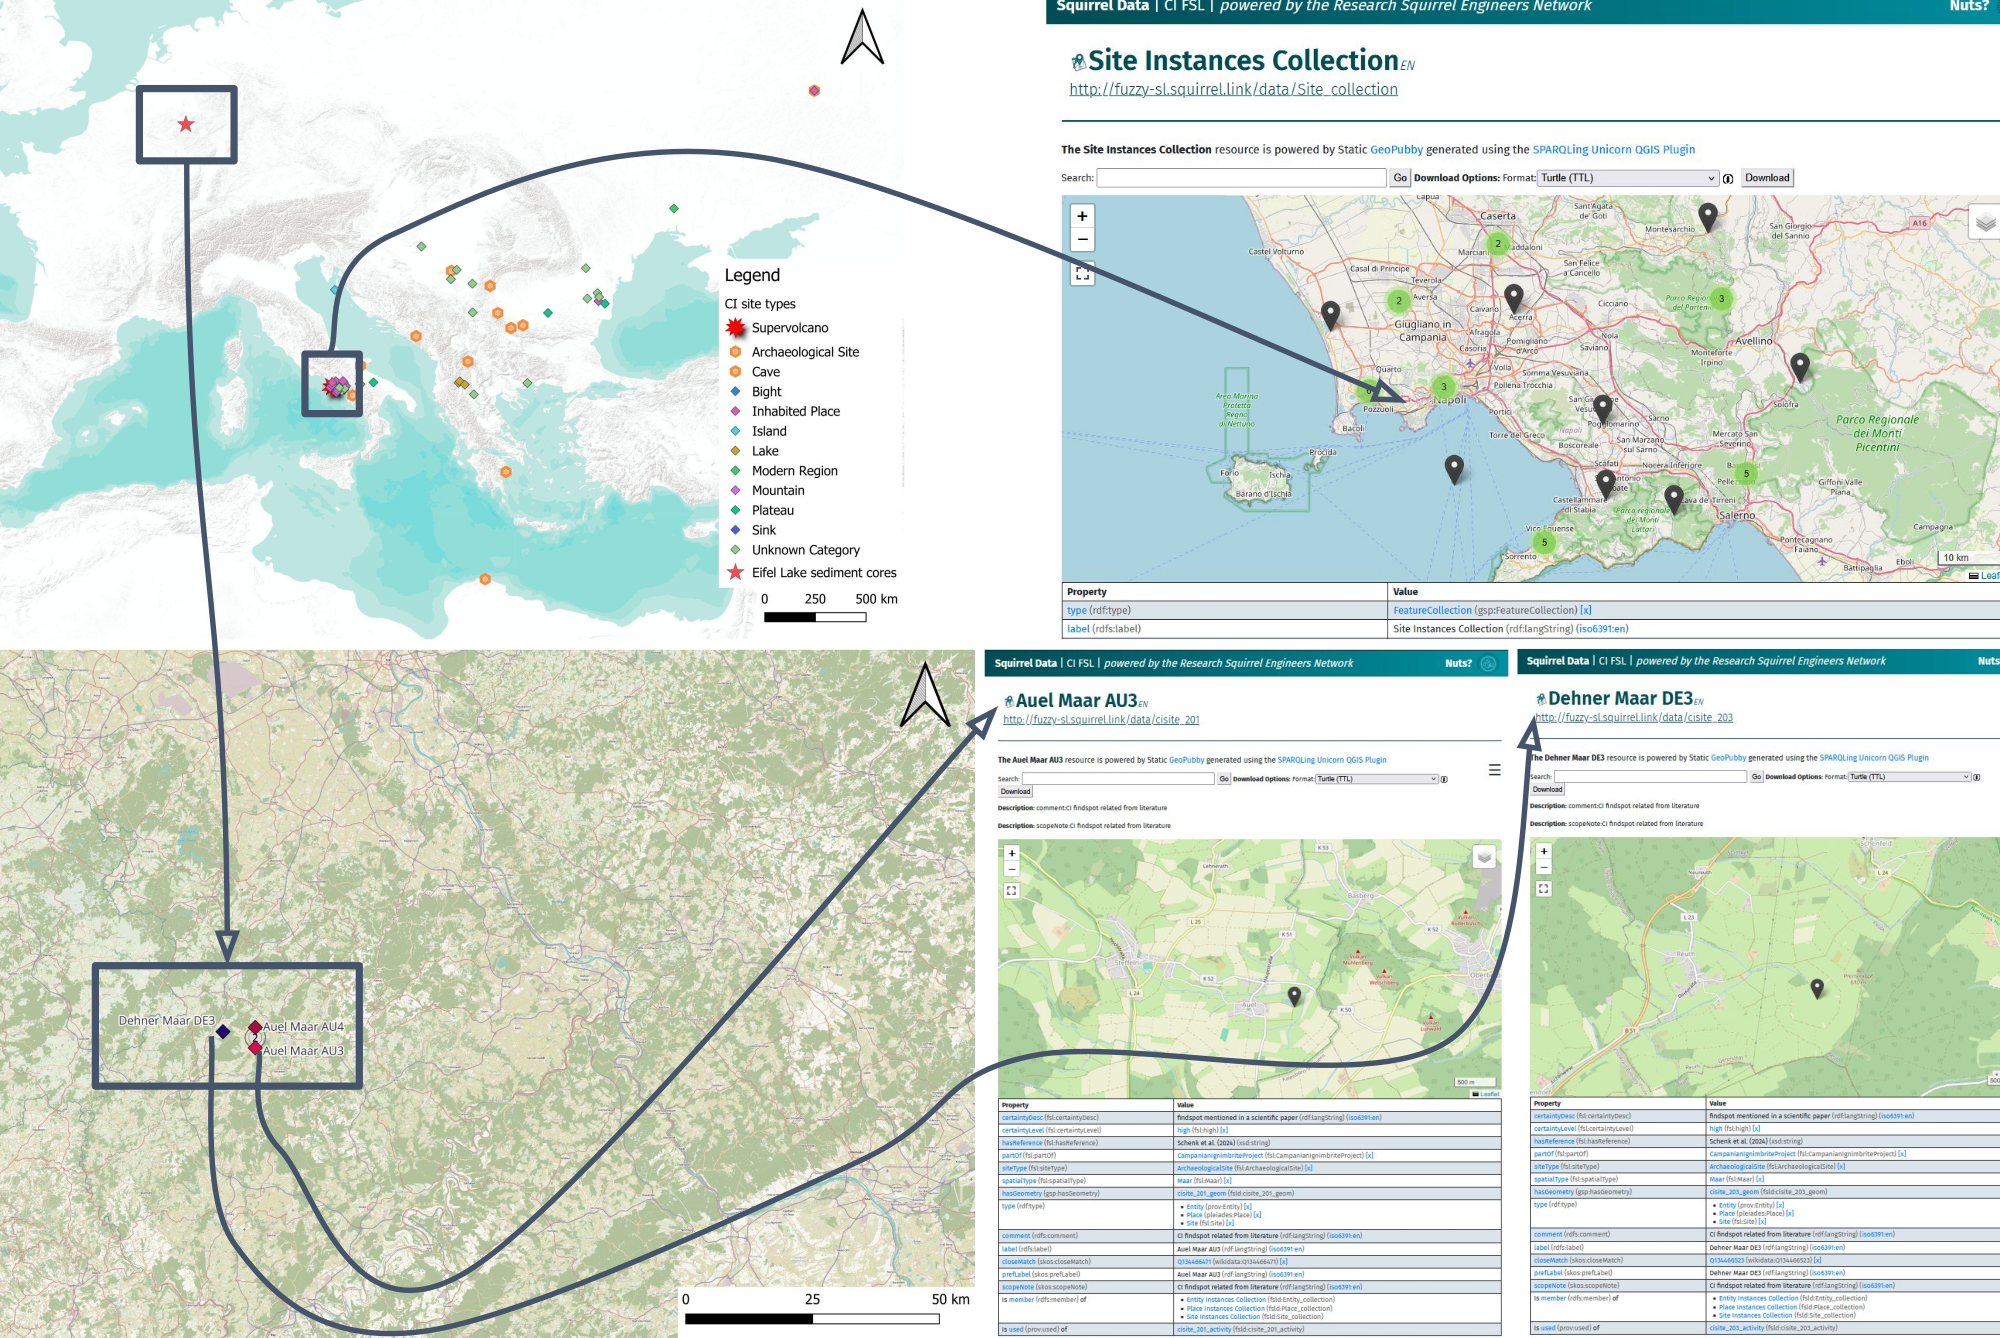
\includegraphics[width=0.95\linewidth]{ECEASST-LaTeX-Templates/img/Campanian Ignimbrite LOD Eifel.png}
    \caption{Campanian Ignimbrite (CI) sites created using the SPARQLing Unicorn Research Toolkit with findspots from~\cite{schenk_cryptotephra_2024,thiery_modelling_2023} CC BY 4.0, Florian Thiery \& Fiona Schenk.}
    \label{fig:unicorn_ci}
\end{figure}

\paragraph{The SPARQLing Unicorn as FAIRification Tool in Computational Archaeology.} From a Research Software Engineering perspective, the toolkit plays a dual role: it is both an enabler of FAIRification workflows and an open research artefact in its own right. The QGIS Plugin and HTML Generator implement the FAIR4RS principles by:

\begin{itemize}
    \item \textbf{Findable}: Each object has a unique URI and is indexed via HTML pages and triplestores
    \item \textbf{Accessible}: publishing RDF and HTML representations in openly available GitHub repositories
    \item \textbf{Interoperable}: The toolkit supports CIDOC CRM, GeoSPARQL, and Wikidata-aligned models
    \item \textbf{Reusable}: Data, code, and workflows are versioned, licensed, and community-documented
\end{itemize}

The toolkit offers a reusable, lightweight solution for semantic integration, especially in disciplines where observational data must be contextualised semantically, such as palaeoclimatology or environmental archaeology. Its modular design encourages domain specialists to adapt and extend its functionality, while retaining core FAIR-compliant structures. This shows how grassroots RSE approaches, grounded in fundamental research needs, can generate sustainable components that contribute to national and international infrastructures such as NFDI or EOSC, while remaining directly usable in everyday domain work. The SPARQLing Unicorn Toolkit exemplifies a domain-tailored FAIRification service, developed at the intersection of community-driven research and infrastructural experimentation. By providing tools for querying, transforming, documenting, and visualising RDF-based Linked Open Data in a GIS-native and semantically compliant way, the toolkit bridges the gap between abstract knowledge graph infrastructures and the practical workflows of archaeological research. In Computational Archaeology, where research data often stems from analogue fieldwork, heterogeneous documentation formats, and legacy databases, semantic integration is essential to ensure long-term accessibility and interoperability. The toolkit supports FAIRification by: enabling the transformation of spatial and contextual data into RDF aligned with CIDOC CRM and GeoSPARQL, generating machine-readable and human-readable documentation (e.g. GitHub-hosted HTML pages), enabling the integration of triplestores and Solid Pods into QGIS, an established environment in archaeology and geosciences and embedding metadata and licensing in a structured, reproducible format. As such, the toolkit advances not only the FAIRness of the data but also the sustainability and transparency of research software in line with FAIR4RS principles. It acts as a reproducible demonstrator and practical enabler for archaeological data producers seeking integration into larger semantic infrastructures (e.g. NFDI4Objects, Base4NFDI).

\paragraph{Challenges and Limitations in the Light of REAL.} While the SPARQLing Unicorn Toolkit substantially contributes to the FAIRification of archaeological and geoscientific data, it also reveals important challenges when assessed against the REAL principles (Reproducible, Executable, Attributable, Literal):

\begin{itemize}
    \item \textbf{Reproducibility}: Query results can vary depending on the state of the endpoint (e.g. Wikidata edits, downtime, schema changes) or QGIS version, which affects plug-in behaviour. Re-executing the same query may yield different outputs after only a few months.
    \item \textbf{Executability}: The toolkit relies on local QGIS installations and external Python dependencies (e.g. rdflib, requests), requiring careful environment management or packaging (e.g. via conda or Docker) to ensure stability across systems and time.
    \item \textbf{Attributability}: While the GitHub-hosted documentation includes links to source datasets and contributors (e.g. Q-IDs, GND, DOIs), attribution of intermediate transformation logic and user-modified layers remains a grey area.
    \item \textbf{Literalness}: The toolkit’s transformation logic (e.g. vector-to-RDF conversion) is transparent in code but often not granularly documented in terms of ontological rationale, especially for non-specialist users.
\end{itemize}

These challenges highlight the broader tension between tool flexibility and reproducibility in applied semantic workflows. As a grassroots, community-maintained project, the SPARQLing Unicorn Toolkit embodies a pragmatic balance: it is not a black-box application, but rather an evolving set of modular tools, whose sustainability depends on openness, user feedback, and shared development responsibility. Despite these limitations, the toolkit provides a blueprint for how FAIRification can be embedded into everyday archaeological practice, without requiring centralised platforms or heavyweight infrastructure. It shows how Research Software Engineering in the humanities can be both FAIR-aware and domain-sensitive.

\subsection{Jupyter Python Minions}\label{sec:33}

As the Semantic Web grows into a vast ecosystem of interlinked knowledge graphs, its potential for archaeological and cultural heritage research increases dramatically. Triplestores like the NFDI4Objects Knowledge Graph, Wikibase instances like Wikidata, and Solid Pods for geoscientific and environmental datasets open new possibilities for interdisciplinary and data-driven research. Yet, while data availability is no longer the main bottleneck, challenges remain: querying these datasets requires SPARQL literacy, and results often arrive in formats not readily compatible with research workflows in archaeology or the digital humanities. To address this gap, the Jupyter Python Minions were developed as part of the SPARQLing Unicorn Research Toolkit by the Research Squirrel Engineers Network. The Minions provide an open-source, lightweight, and modular Python interface to simplify SPARQL querying, data transformation, and visualisation in a Jupyter environment. The goal is to lower the entry barrier for archaeologists and domain researchers with limited programming experience while maintaining compliance with FAIR and FAIR4RS principles. Using Jupyter Notebooks as the delivery format offers several advantages:

\begin{itemize}
    \item \textbf{Transparency}: complete workflows (from query to output) are documented and shareable
    \item \textbf{Reproducibility}: queries, visualisations, and transformations are embedded and executable
    \item \textbf{Modularity}: functions can be reused, adapted, and extended across domains
    \item \textbf{Community adaptability}: Notebooks can be published on GitHub, archived via Zenodo, and reused in training or infrastructure contexts (e.g. Jupyter4NFDI)
\end{itemize}

The Minions support federated queries and local endpoints and can output results as pandas DataFrames for further processing. This workflow has been demonstrated in multiple archaeological and geoscientific use cases:

\paragraph{Use Case 1 – Ogham Stones.} In this use case, SPARQL queries were executed against Wikidata and the NFDI4Objects Knowledge Graph to retrieve data on early medieval Ogham stones in Ireland. Jupyter Minions were used to extract metadata (e.g. inscription content, certainty, typology), generate distribution charts (e.g. stone types by county) and produce interactive maps visualising findspots (Figure~\ref{fig:minion}). Relevant notebooks: are Wikidata Ogham Sites Map\footnote{cf. \url{https://research-squirrel-engineers.github.io/jupyter-nb-lod/wikidata-ogham-sites-map}}, NFDI4Objects Ogham Sites per County\footnote{cf. \url{https://research-squirrel-engineers.github.io/jupyter-nb-lod/n4okg-ogham-sites-county}} and NFDI4Objects Ogham Map\footnote{cf. \url{https://research-squirrel-engineers.github.io/jupyter-nb-lod/n4okg-ogham-sites-maps}}.

\paragraph{Use Case 2 – Samian Ware: Roman ceramic production sites (especially Samian kiln sites) are well-represented in Wikidata.} Using Jupyter Python Minions, these were queried and grouped by production region or typological classification, producing bar charts and tabular outputs. Notebook: Wikidata Samian Kilnsites\footnote{cf. \url{https://research-squirrel-engineers.github.io/jupyter-nb-lod/wikidata_samian_kilnsites}}.

\paragraph{Use Case 3 – Campanian Ignimbrite.} This interdisciplinary use case connects geoscience and archaeology by retrieving findspots of CI tephra layers from a Solid Pod, with geospatial and statistical visualisations in Jupyter. The workflow includes: querying RDF-based site data and tephra evidence, generating diagrams and summary tables and rendering interactive dispersal maps. Notebook: SolidPod CI Dataset\footnote{cf. \url{https://research-squirrel-engineers.github.io/jupyter-nb-lod/solidpod-ci}}.

\begin{figure}[h!]
    \centering
    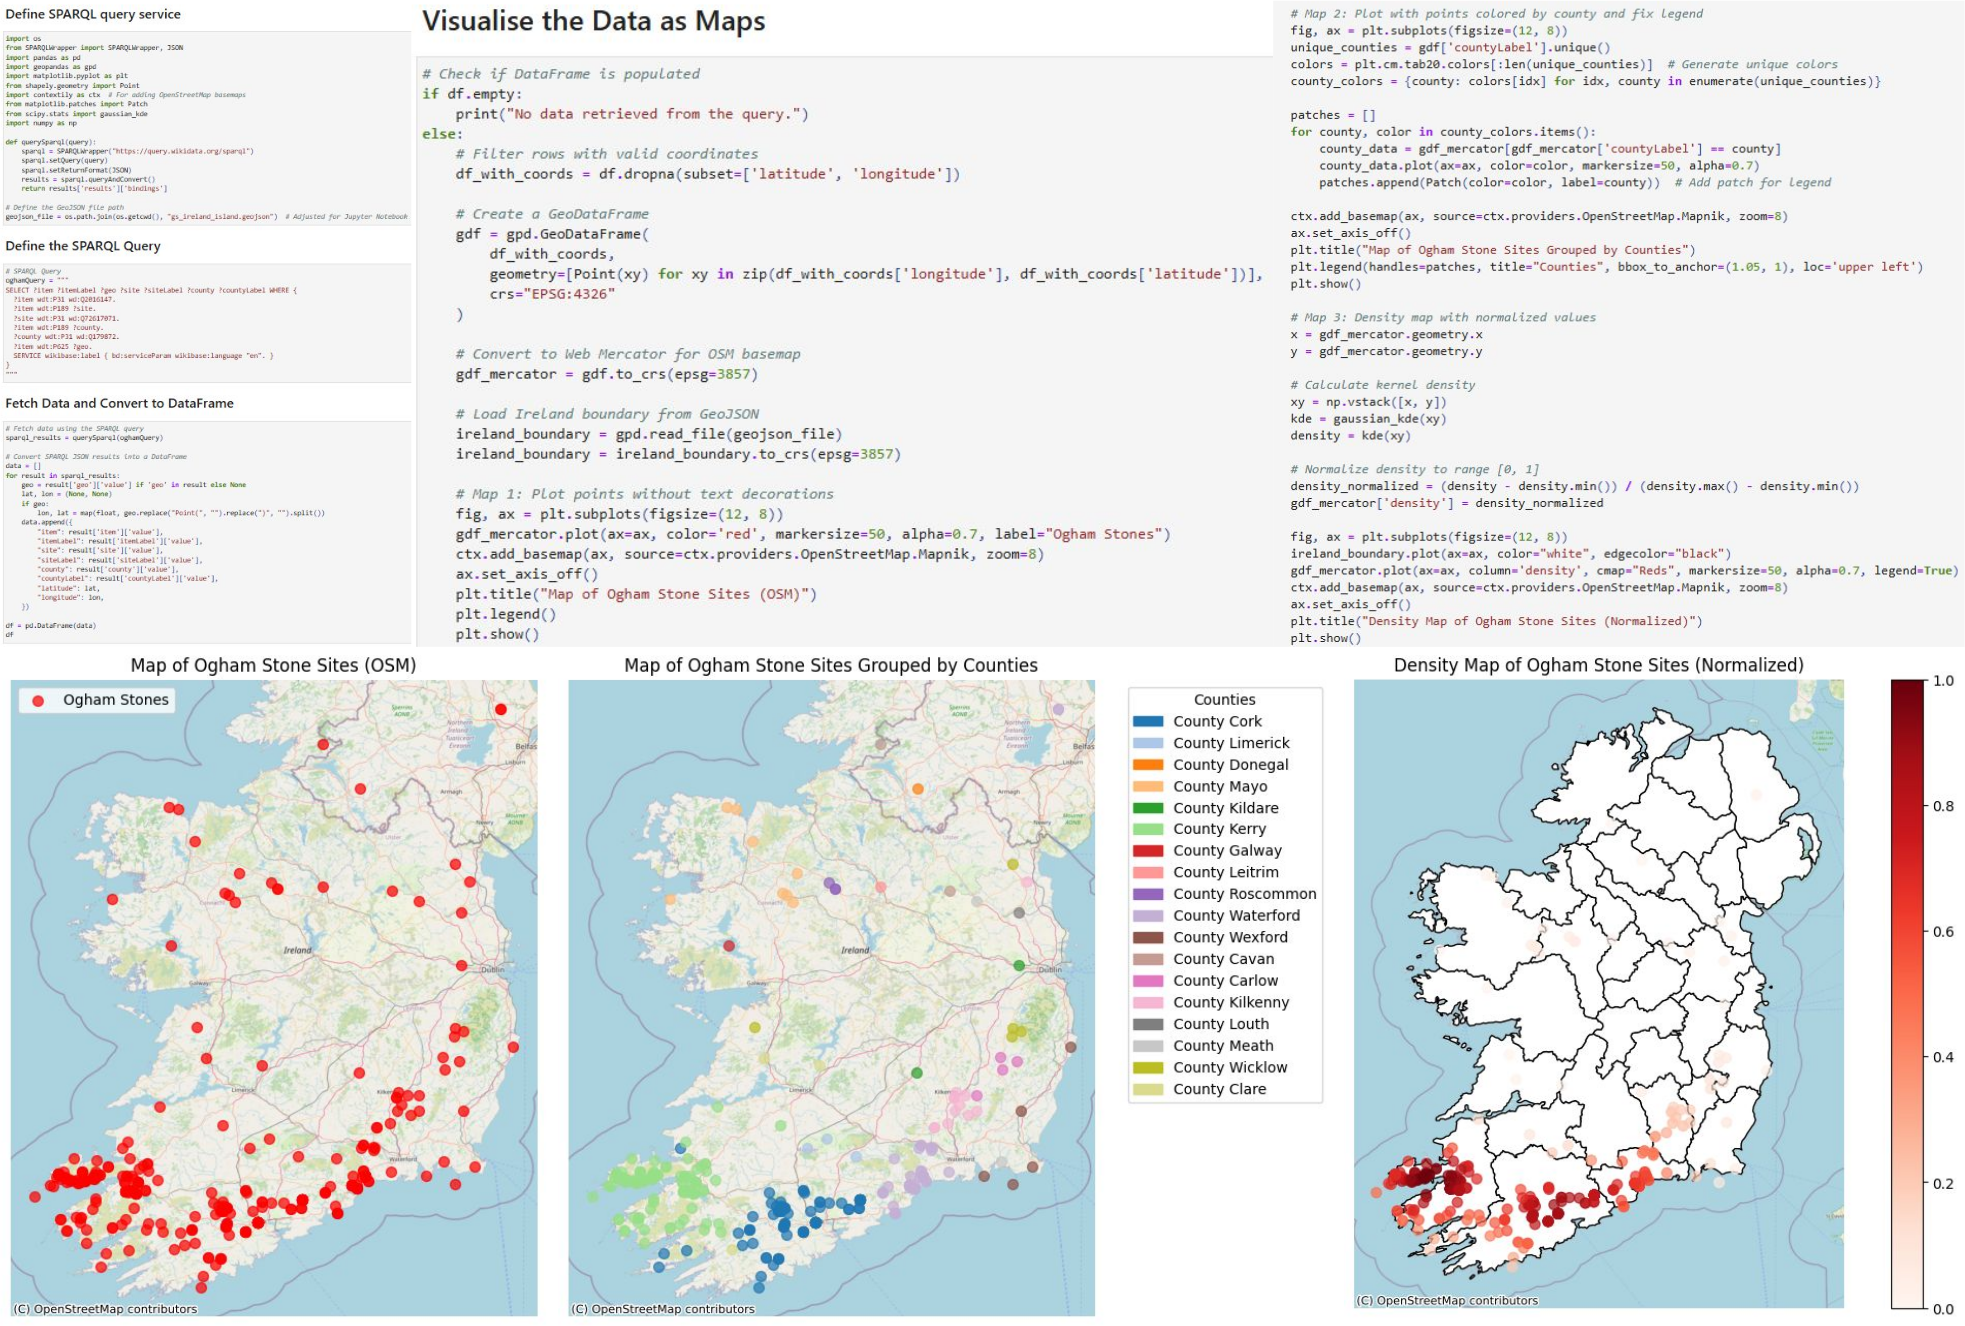
\includegraphics[width=0.95\linewidth]{ECEASST-LaTeX-Templates/img/Python Minions.png}
    \caption{Ogham Visualisations using a Python Jupyter Minion. Florian Thiery, CC BY 4.0.}
    \label{fig:minion}
\end{figure}

\paragraph{Jupyter Minions as FAIRification Tools in Computational Archaeology.} The Jupyter Python Minions function as modular FAIRification helpers that embed semantic querying and RDF processing directly into computational workflows. They are especially relevant in Computational Archaeology, where the digital transformation of analogue legacy data often lacks structured formats and machine-actionable metadata. By integrating RDF, SPARQL, and visualisation within a single executable research object, the Minions address several core FAIRification challenges: (i) they standardise the access and transformation of semantically modelled archaeological data, (ii) they enable reproducible data visualisation, which is often fragmented across multiple tools, (iii) they facilitate cross-domain interoperability between the humanities, geosciences, and environmental data ecosystems, they support the creation of FAIR Digital Objects (FDOs) in a notebook-native context. As a result, these Minions not only support domain researchers in producing FAIR data but also help ensure that the research software remains FAIR: documented, versioned, openly licensed, and linked to persistent identifiers via platforms like Zenodo and GitHub.

\paragraph{Challenges and Limitations in the Light of REAL. } Despite their strengths, the use of Jupyter Notebooks and Minions also reveals significant limitations, particularly concerning the REAL principles discussed in section 2:

\begin{itemize}
    \item \textbf{Reproducibility}: While the code and data may remain stable, endpoint changes (e.g. Wikidata schema evolution, endpoint availability) can lead to divergent results over time.
    \item \textbf{Executability}: Dependencies in Python environments (e.g. pandas, rdflib, SPARQLWrapper) may cause notebooks to fail without proper containerisation or virtualisation.
    \item \textbf{Attributability}: While the Minions encourage citation via DOI and Zenodo export, linking to the original data sources and contributors (e.g. Wikidata editors) remains complex.
    \item \textbf{Literalness}: The transparency of the workflow is clear in notebook logic, but more complex RDF transformation steps often remain opaque for users not trained in SPARQL or semantic modelling.
\end{itemize}

These limitations reflect broader challenges in computational heritage science: while notebooks foster openness and reusability, accurate reproducibility is constrained by a dynamic technological landscape and a dependence on externally hosted, often community-maintained endpoints. Nonetheless, the Minions represent a pragmatic, community-driven solution: they offer reproducible workflows "good enough" for many scholarly purposes. They make semantic FAIRification tangible and teachable in various research and educational contexts.

\section{Discussion}\label{sec:discussion}

The preceding chapters have outlined how domain-specific Research FAIRification Tools (RFAIRTs), developed by a grassroots community, support semantic interoperability and promote FAIR data and software practices in Computational Archaeology and beyond. This discussion reflects on the broader implications of such an approach, focusing on tensions and synergies between community-driven Research Software Engineering (RSE), the FAIR4RS principles, and the previously introduced REAL framework. Although the Research Squirrel Engineers Network operates outside formal institutional structures, its tools and methodologies align closely with the objectives of national infrastructure initiatives such as the German National Research Data Infrastructure (NFDI). Rather than competing, the network complements existing infrastructures by contributing modular, standards-compliant tools like the SPARQLing Unicorn Plugin and the Jupyter Python Minions. It also supports the expansion of basic services such as Jupyter4NFDI and nfdi.software, and facilitates integration of semantic data into the NFDI Knowledge Graph Infrastructure (KGI4NFDI). This constellation illustrates a productive tension between agility and sustainability. Community-developed tools are typically closer to research questions and more adaptable to domain-specific needs, while infrastructure-driven services offer long-term availability, technical robustness, and persistent identifiers. Ensuring interoperability between both layers is crucial: grassroots software must become infrastructure-ready without losing its epistemic grounding in specific disciplinary workflows.

Sustainability remains a core challenge. FAIRification is not a single event but an ongoing process requiring maintenance, community engagement, and institutional recognition. While the tools described here are openly licensed, version-controlled, and documented, their long-term viability depends on an ecosystem of contributors, trainers, reviewers, and users. This necessitates social infrastructure beyond code: active documentation, support channels, developer onboarding, and crediting mechanisms – especially in interdisciplinary and citizen science projects where traditional authorship norms fall short. Comparing the FAIR4RS principles and the REAL framework highlights a second set of tensions. While FAIR4RS ensures software is findable, accessible, interoperable, and reusable, the REAL dimensions probe deeper into scientific credibility and practical usability. The tools discussed here are clearly FAIR – openly published, semantically structured, and interoperable by design. Their REALness, however, is more situational and contingent. Reproducibility may suffer from changing SPARQL endpoints, QGIS plugin versions, or Python package dependencies. Executability is not always guaranteed unless tools are containerised or bound to stable environments. Attribution is partly ensured through persistent identifiers and Zenodo archiving, but the provenance of internal logic – such as SPARQL queries or transformation pipelines – is harder to preserve. Literalness remains especially challenging: while internal workings are exposed, modelling assumptions are rarely explicit, especially when GUI abstractions or default mappings are used. These limitations do not diminish the tools’ value but clarify the limits and expectations of reusable RSE in the humanities. The interdisciplinary potential of RFAIRTs is illustrated by the Campanian Ignimbrite example. Although developed in an archaeological setting, the same tools proved effective for geoscientific data FAIRification, linking tephra records from maar lakes with volcanic chronologies and archaeological cave sites. This shows that lightweight, modular semantic tools can enable cross-disciplinary integration – provided that domain-specific ontologies, data structures, and use cases are respected. Transferability depends less on technical generality than on shared practices of semantic negotiation and FAIRification logic.

Finally, the tools introduced here serve both didactic and epistemic functions. By revealing semantic relationships, data provenance, and transformation workflows, they allow students and researchers to interrogate and adapt digital methods transparently. Notebooks and GIS projects become executable research articles – living documents of method and model. In this regard, the RFAIRT approach promotes not only Open Science, but also Open Interpretation: embedding FAIRification into the research process itself, rather than treating it as a post hoc standardisation step.

\section{Conclusion and Outlook}
\label{sec:conclusion}

This paper presents a best-practice case study of research software engineering within computational archaeology, demonstrating how community-driven tools can enable FAIR data and FAIR4RS-compliant research software. The development and use of the SPARQLing Unicorn Research Toolkit and the Jupyter Python Minions show that lightweight, modular FAIRification services can emerge from grassroots initiatives and still integrate effectively with national research infrastructures such as the NFDI. The experiences discussed underline that semantic FAIRification is not limited to data alone – it also applies to research workflows, ontological modelling, and code itself. The community-oriented development philosophy of the Research Squirrel Engineers Network exemplifies how sustainable RSE can be embedded within domain-specific contexts while contributing to broader Open Science goals. However, this approach also reveals unresolved challenges. Ensuring reproducibility and long-term executability of research software remains difficult, especially in dynamic environments like Wikidata or Solid Pods. Attribution and transparency require deliberate design choices, and the literalness of code in relation to conceptual models often remains implicit. Despite these limitations, the tools and practices presented here offer a viable pathway for FAIRification in other domains. Their successful application to both archaeological and geoscientific data suggests that well-designed, community-sustained RFAIRTs can support interoperability across disciplines. Moving forward, closer alignment with infrastructure initiatives, through containerisation, metadata standardisation, and inclusion in services like nfdi.software, can further enhance their impact and sustainability. By continuing to combine openness, semantic rigour, and practical usability, the community-based RSE approach in Computational Archaeology can serve as a valuable reference model for other fields working at the intersection of data, software, and cultural knowledge.

\begin{acknowledge}
This paper is part of the DFG-funded NFDI initiative, specifically the Research Data Infrastructure for the Material Remains of Human History (NFDI4Objects), DFG Project number 501836407. Some works were funded by Wikimedia Deutschland, Fellow-Programm Freies Wissen 2020/21: “Irische Ogham Steine im Wikimedia Universum”. The authors acknowledge the use of language assistance powered by artificial intelligence (ChatGPT, OpenAI) for stylistic editing and linguistic refinement. All content and arguments were authored and verified by the authors themselves.
\end{acknowledge}

\nocite{*}
\bibliographystyle{eceasst}
\bibliography{references}

\end{document}
